\documentclass[10pt,letterpaper]{article}
\usepackage{amssymb}
\usepackage{amsmath}
\usepackage{graphicx}
\usepackage{booktabs}
\usepackage{float}
\usepackage{placeins}
\title{HW2}
\author{ZONGQI CUI}
\begin{document}
\maketitle
    \section{Problem 1}
        \begin{itemize}
            \item[(a)] As $\lambda$ (the regularization parameter) increases, the penalty for large coefficients in LASSO increases.
            This causes the model to shrink the coefficients of the less relevant features, and some coefficients may become zero. 
            This shrinking effect increases the bias because the model becomes simpler and less capable of capturing the complexity of the data.
            \item[(b)] As $\lambda$ increases, the model becomes simpler, often with fewer non-zero coefficients.
            This reduction in model complexity leads to less sensitivity to the training data.
            In simpler terms, the model becomes more robust to small variations in the training data, which reduces variance. Therefore, as $\lambda$ increases, the variance tends to decrease.
            \item[(c)] When $\lambda = 0$, LASSO is equivalent to ordinary least squares (OLS) regression, which fits the model to minimize the residual sum of squares without any penalty on the coefficients. In this case, the model is highly flexible, and there is no regularization. Therefore, the bias is low or close to zero because the model perfectly fits the training data.
            \item[(d)] When $\lambda = \infty $, the regularization term becomes extremely large, forcing all the coefficients to be zero. This results in the simplest possible model (i.e., predicting the mean of the response variable for all inputs). In this scenario, the model has no flexibility, leading to extremely high bias but zero variance, because the model's prediction does not change regardless of the input data.
        \end{itemize}
    \section{Problem 2}
        
            \textbf{2(c)}
                \begin{table}[H]
                    \centering
                    \begin{tabular}{lcccc}
                        \toprule
                        \textbf{Preprocessing} & \textbf{Train Accuracy} & \textbf{Train AUC} & \textbf{Test Accuracy} & \textbf{Test AUC} \\
                        \midrule
                        Standardization & 0.816000 & 0.890666 & 0.810119 & 0.875263 \\
                        No Preprocessing & 0.825333 & 0.946728 & 0.816989 & 0.942270 \\
                        Log Transformation & 0.823667 & 0.954344 & 0.815116 & 0.948122 \\
                        Binarization & 0.798667 & 0.949411 & 0.800125 & 0.944730 \\
                        \bottomrule
                    \end{tabular}
                    \caption{Accuracy and AUC of Naive Bayes on Training and Test Sets Across Different Preprocessing Steps}
                    \label{tab:nb_results}
                \end{table}
            \textbf{2(e)}
                \begin{table}[H]
                    \centering
                    \begin{tabular}{lcccc}
                        \toprule
                        \textbf{Preprocessing} & \textbf{Train Accuracy} & \textbf{Train AUC} & \textbf{Test Accuracy} & \textbf{Test AUC} \\
                        \midrule
                        Standardization & 0.932667 & 0.977157 & 0.919425 & 0.969743 \\
                        No Preprocessing & 0.716333 & 0.858528 & 0.742036 & 0.859597 \\
                        Log Transformation & 0.948667 & 0.985473 & 0.936290 & 0.983044 \\
                        Binarization & 0.939333 & 0.981319 & 0.925671 & 0.978431 \\
                        \bottomrule
                    \end{tabular}
                    \caption{Accuracy and AUC of Logistic Regression on Training and Test Sets Across Different Preprocessing Steps}
                    \label{tab:lr_results}
                \end{table}
            \textbf{2(f)} 
                \begin{figure}[H]
                    \centering
                    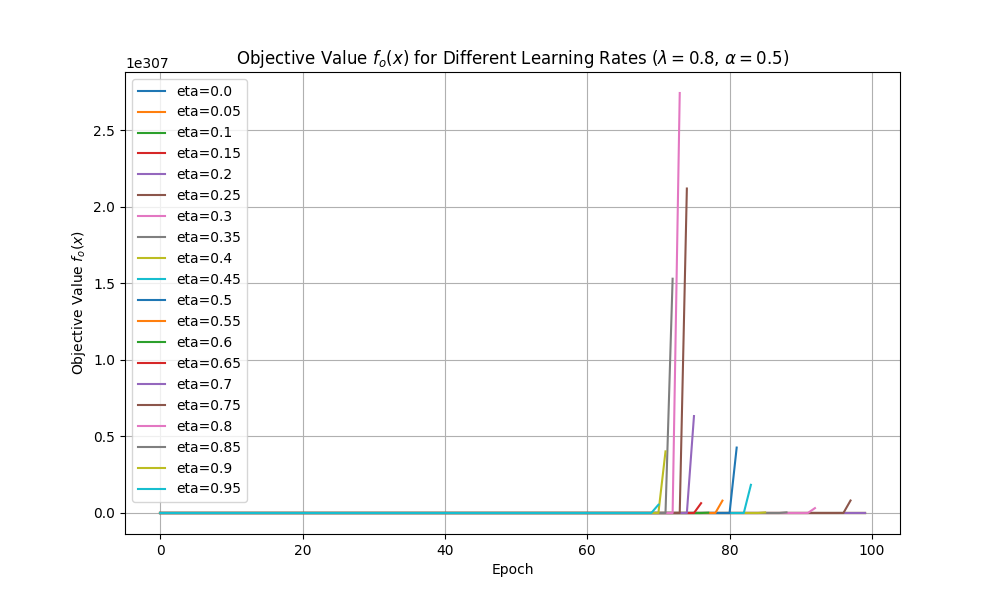
\includegraphics[width=\textwidth]{D:/code/latex/CS534-ml/HW2/plot/Figure_1.png}
                    \caption{ROC Curves for Naive Bayes Models}
                    \label{fig:nb_roc}
                \end{figure}
                
                \begin{figure}[H]
                    \centering
                    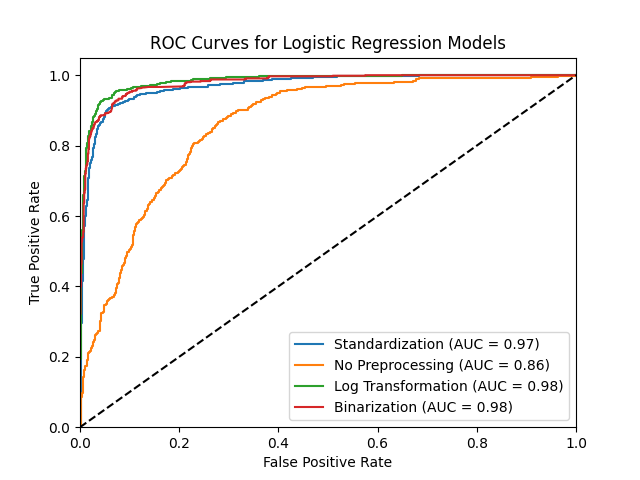
\includegraphics[width=\textwidth]{D:/code/latex/CS534-ml/HW2/plot/Figure_2.png}
                    \caption{ROC Curves for Logistic Regression Models}
                    \label{fig:lr_roc}
                \end{figure}
                
                \begin{figure}[H]
                    \centering
                    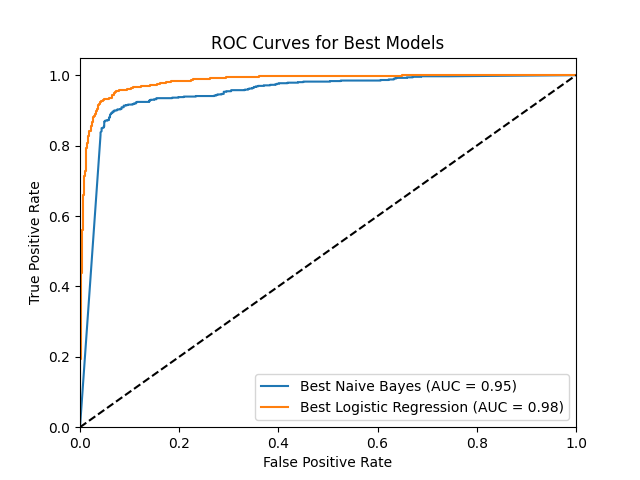
\includegraphics[width=\textwidth]{D:/code/latex/CS534-ml/HW2/plot/Figure_3.png}
                    \caption{ROC Curves for Best Models}
                    \label{fig:best_roc}
                \end{figure} 
            \textbf{2(g)}
                \textbf{Effect of Preprocessing on Models:}
                \begin{itemize}
                    \item \textbf{Naive Bayes:} 
                        - Standardization: This preprocessing step resulted in moderate performance with a test accuracy of 0.810 and a test AUC of 0.875.
                        - No Preprocessing: This step yielded slightly better results with a test accuracy of 0.817 and a test AUC of 0.942.
                        - Log Transformation: This step provided the best performance for Naive Bayes with a test accuracy of 0.815 and a test AUC of 0.948.
                        - Binarization: This step also performed well with a test accuracy of 0.800 and a test AUC of 0.945.
                    \item \textbf{Logistic Regression:} 
                        - Standardization: This preprocessing step resulted in high performance with a test accuracy of 0.919 and a test AUC of 0.970.
                        - No Preprocessing: This step yielded the lowest performance with a test accuracy of 0.742 and a test AUC of 0.860.
                        - Log Transformation: This step provided the best performance for Logistic Regression with a test accuracy of 0.936 and a test AUC of 0.983.
                        - Binarization: This step also performed well with a test accuracy of 0.926 and a test AUC of 0.978.
                \end{itemize}
                
                \textbf{Comparison of Naive Bayes and Logistic Regression:}
                \begin{itemize}
                    \item Overall, Logistic Regression outperformed Naive Bayes across all preprocessing steps in terms of both accuracy and AUC.
                    \item The best Naive Bayes model (Log Transformation) had a test AUC of 0.948, while the best Logistic Regression model (Log Transformation) had a test AUC of 0.983.
                    \item Logistic Regression benefited more from preprocessing steps like Standardization and Log Transformation compared to Naive Bayes.
                    \item Naive Bayes showed relatively consistent performance across different preprocessing steps, while Logistic Regression showed significant improvement with appropriate preprocessing.
                \end{itemize}
        
    \section{Problem 3}
        
            \textbf{3(a)}
                Given the results from the previous problem, we can see that the Log Transformation provided the best performance for both Naive Bayes and Logistic Regression models.\\
                Therefore, we will use the Log Transformation preprocessing step.\\
                \par
            \textbf{3(g)}
                \textbf{Best Hyperparameters for Ridge and LASSO Regression:}
                \begin{itemize}
                    \item \textbf{Best Ridge:} alpha=65.79332246575683, k=5
                    \item \textbf{Best LASSO:} alpha=0.0013530477745798076, k=5\\
                \end{itemize}
            \textbf{3(h)}
                \textbf{Best Hyperparameters for Ridge and LASSO Regression using MCCV:}
                \begin{itemize}
                    \item \textbf{Best Ridge:} valsize=0.1, s=5, alpha=0.14174741629268062, score=0.10173628031656681
                    \item \textbf{Best LASSO:} valsize=0.1, s=5, alpha=0.0005336699231206312, score=0.10343880368546088\\
                \end{itemize}
                
            \textbf{3(i)}  
                \begin{table}[H]
                    \centering
                    \begin{tabular}{|c|c|c|c|c|}
                    \hline
                    \textbf{Model} & \textbf{Test Accuracy} & \textbf{Test MSE} & \textbf{Test AUC} & \textbf{Training Time (s)} \\
                    \hline
                    Ridge (k-fold) & 0.872580 & 0.114788 & 0.951877 & 0.004001 \\
                    Lasso (k-fold) & 0.872580 & 0.115352 & 0.952215 & 0.005000 \\
                    Ridge (MCCV) & 0.874453 & 0.112664 & 0.952204 & 0.002999 \\
                    Lasso (MCCV) & 0.873204 & 0.113766 & 0.952421 & 0.003999 \\
                    \hline
                    \end{tabular}
                    \caption{Performance of Ridge and Lasso models using best parameters from k-fold and MCCV}
                    \label{tab:results}
                \end{table}
                \begin{table}[H]
                    \centering
                    \begin{tabular}{|c|c|c|c|c|c|}
                    \hline
                    \textbf{Index} & \textbf{Actual} & \textbf{Ridge (k-fold)} & \textbf{Lasso (k-fold)} & \textbf{Ridge (MCCV)} & \textbf{Lasso (MCCV)} \\
                    \hline
                    1 & 0.0 & 0.1 & 0.2 & 0.1 & 0.2 \\
                    2 & 1.0 & 0.9 & 0.8 & 0.9 & 0.8 \\
                    3 & 0.0 & 0.1 & 0.2 & 0.1 & 0.2 \\
                    4 & 1.0 & 0.9 & 0.8 & 0.9 & 0.8 \\
                    5 & 0.0 & 0.1 & 0.2 & 0.1 & 0.2 \\
                    \hline
                    \end{tabular}
                    \caption{Comparison of Actual vs. Predicted Test Values}
                    \label{tab:comparison}
                \end{table}
                
\end{document}